\documentclass[../report.tex]{subfiles}

\begin{document}
\subsection{Các dòng vi điều khiển} 
Năm 1980 khi intel tung ra chip 8051, 
bộ vi điều khiển đầu tiên của họ MCS-51 và là chuẩn công nghệ cho 
nhiều họ vi điều khiển được sản xuất sau này.
Năm 1980 Intel công bố chip 8051 (80C51),
bộ vi điều khiển đầu tiên của họ vi điều khiển MCS-51 bao gồm:
\begin{itemize}
\item 4 KB ROM
\item 128 byte RAM
\item 32 đường xuất nhập 
\item 1 port nối tiếp và 2 timer/counter 16 bit
\end{itemize}
Hiện nay, Intel không còn cung cấp các loại 
Vi điều khiển họ MCS-51 nữa, thay vào đó các nhà sản xuất khác như Atmel, 
Philips/signetics, AMD, Siemens, Matra \& Dallas, Semiconductors 
được cấp phép làm nhà cung cấp thứ hai cho các chip của họ MSC-51.

Chip Vi điều khiển được sử dụng rộng rãi trên thế giới cũng như ở Việt Nam hiện nay là Vi điều khiển của hãng Atmel.
Các mã số chip được thay đổi chút ít khi được Atmel sản xuất. 
Mã số 80 chuyển thành 89, chẳng hạn 80C52 của Intel khi sản xuất ở Atmel mã số thành 89C52 (Mã số đầy đủ: AT89C52).
Với tính năng chương trình tương tự như nhau. Tương tự 8051, 8053, 8055 có mã số tương đương ở Atmel là 89C51, 89C53, 89C55.

Sau khoảng thời gian cải tiến và phát triển, 
hãng Atmel tung ra thị trường dòng Vi điều khiển mang số hiệu 89Sxx 
với nhiều cải tiến và đặc biệt là có thêm khả năng nạp chương trình 
theo chế độ nối tiếp rất đơn giản và tiện lợi cho người sử dụng.

Dung lượng RAM Dung lượng ROM Chế độ nạp:
\begin{itemize}
\item 89S51 128 byte 4 Kbyte nối tiếp.
\item 89S52 128 byte 8 Kbyte nối tiếp.
\item 89S53 128 byte 12 Kbyte nối tiếp.
\item 89S55 128 byte 20 Kbyte nối tiếp.
\end{itemize}

Tổng quát thông số kĩ thuật của AT89S52: 
\begin{itemize}
\item 8 KB bộ nhớ có thể lập trình nhanh, có khả năng tới 1000 chu kỳ ghi/xoá.
\item Tần số hoạt động từ: 0Hz đến 24 MHz
\item 3 mức khóa bộ nhớ lập trình
\item 3 bộ Timer/counter 16 Bit
\item 128 byte RAM nội.
\item 4 port xuất /nhập I/O 8 bit.
\item Giao tiếp nối tiếp.
\item 64 KB vùng nhớ mã ngoài
\item 64 KB vùng nhớ dữ liệu ngoại.
\item $4\mu s$ cho hoạt động nhân hoặc chia
\end{itemize}

\subsection{Các chân của AT89S52}
\begin{figure}[H]
\centering
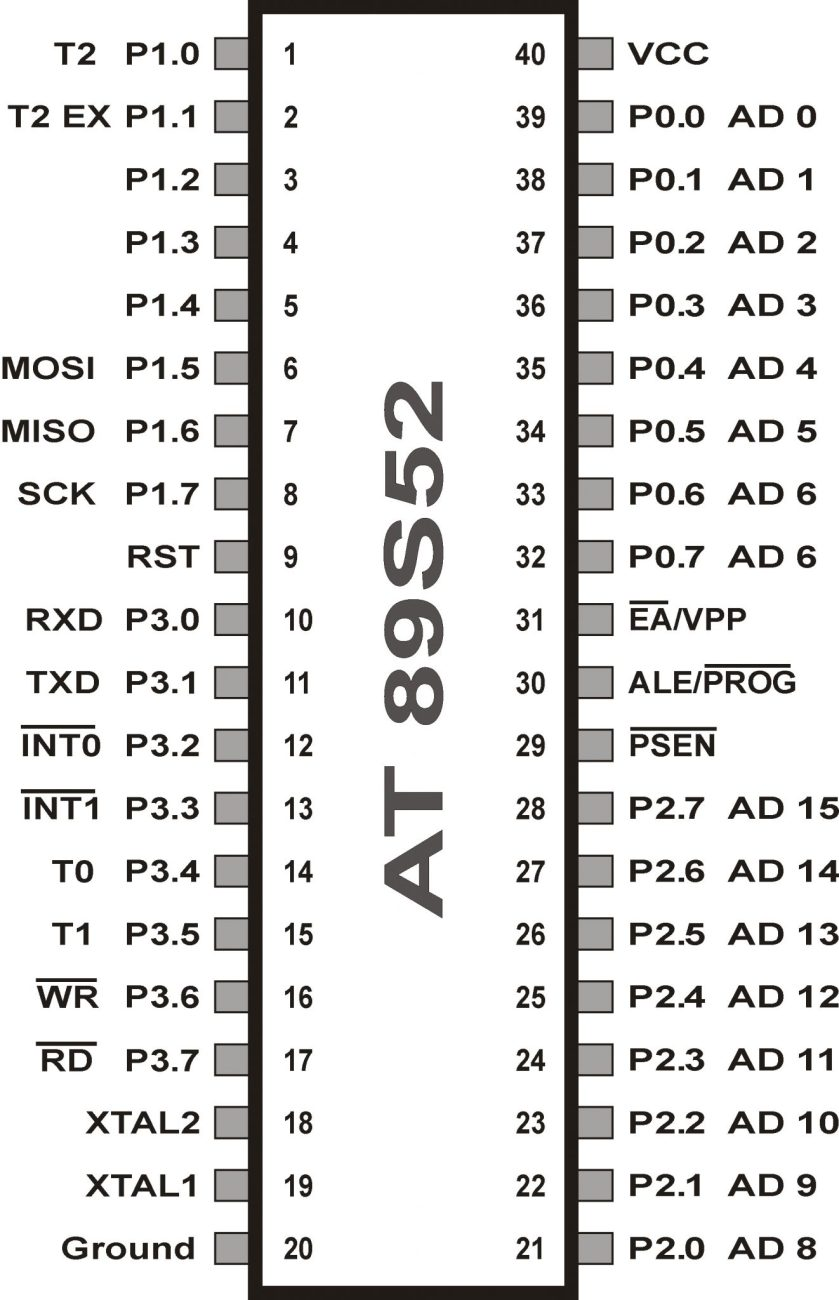
\includegraphics[width=6cm]{figures/at89s52_pins.jpg}
\caption{Sơ đồ chân}
\end{figure}

\begin{itemize}
\item Nhóm chân nguồn: 
\begin{itemize}
\item VCC: chân 40, điện áp cung cấp 5V DC.
\item GND: chân 20.
\end{itemize}

\item Nhóm chân dao động: Gồm chân 18 và chân 19 (XTAL2 và XTAL1), cho phép 
ghép nối thạch anh vào mạch dao động bên trong vi điều khiển, được sử dụng để nhận nguồn xung 
clock từ bên ngoài để dao động, thường được ghép nối với thạch anh và các tụ để tạo nguồn xung clock ổn định. 
\begin{itemize}
\item XTAL1: ngõ vào đến mạch khuếch đại dao động đảo và ngõ vào đến mạch tạo dao động xung clock bên trong. 
\item XTAL2: Ngõ ra từ mạch khuếch đại dao động đảo. 
\end{itemize}

\item Chân chọn bộ nhớ chương trình: chân 31 (EA/VPP) dùng để xác định chương trình thực hiện 
được lấy từ ROM nội hay ROM ngoại. 
\begin{itemize}
\item Chân 31 nối đất: sử dụng bộ nhớ bên ngoài. 
\item Chân 31 nối nguồn: sử dụng bộ nhớ chương trình (4KB) bên trong vi điều khiển. 
\end{itemize}

\item RST(chân reset): chân 9 dùng để thiết lập trạng thái ban đầu cho vi điều khiển. 
\item Chân cho phép bộ nhớ chương trình PSEN: PSEN (program store enable) tsin hiệu được xuất 
ra ở chân 29 dùng để truy xuất bộ nhớ chương trình ngoài. Chân này thường được nối với chân OE 
(output enable) của ROM ngoài. 
Khi vi điều khiển làm việc với bộ nhớ chương trình ngoài, 
chân này phát ra tín hiệu kích hoạt ở mức thấp và được kích hoạt 2 lần trong một chu kì máy.
Khi thực thi một chương trình ở ROM nội, 
chân này được duy trì ở mức logic không tích cực (logic 1).

\item Chân ALE: chân 30, chốt địa chỉ. 
Khi Vi điều khiển truy xuất bộ nhớ từ bên ngoài, 
port 0 vừa có chức năng là bus địa chỉ, 
vừa có chức năng là bus dữ liệu do đó phải tách các đường dữ liệu và địa chỉ. 
Tín hiệu ở chân ALE dùng làm tín hiệu điều khiển để giải đa hợp các đường địa chỉ 
và các đường dữ liệu khi kết nối chúng với IC chốt.

\item Nhóm chân điều khiển vào/ra: 
\begin{itemize}
\item Port 0, gồm 8 chân (từ chân 32 đến 39) có hai chức năng:
\begin{itemize}
    \item Chức năng xuất/nhập: các chân này được dùng để nhận tín hiệu từ bên ngoài vào để xử lí, 
    hoặc dùng để xuất tín hiệu ra bên ngoài, chẳng hạn xuất tín hiệu để điều khiển led đơn sáng tắt.
    \item Chức năng là bus dữ liệu và bus địa chỉ (AD7-AD0): 8 chân này (hoặc Port 0) còn làm nhiệm vụ 
    lấy dữ liệu từ ROM hoặc RAM ngoại (nếu có kết nối với bộ nhớ ngoài), 
    đồng thời Port 0 còn được dùng để định địa chỉ của bộ nhớ ngoài.
\end{itemize}

\item Port 1, gồm 8 chân (từ chân 1 đến chân 8) chỉ có chức năng làm các đường xuất/nhập, không có chức năng khác.
\item Port 2, gồm 8 chân (từ chân 21 đến chân 28) có hai chức năng:
\begin{itemize}
\item Chức năng xuất/nhập
\item Chức năng là bus địa chỉ cao (A8-A15): khi kết nối với bộ nhớ ngoài có dung lượng lớn,
cần 2 byte để định địa chỉ của bộ nhớ, byte thấp do P0 đảm nhận, byte cao do P2 này đảm nhận.
\end{itemize}
\item Port 3, gồm 8 chân (từ chân 10 đến 17) với chức năng chính xuất/nhập.
\end{itemize}
\item Các chức năng khác: 
\begin{itemize}
\item P3.0 RxD: Ngõ vào nhận dữ liệu nối tiếp. 
\item P3.1 TxD: Ngõ xuất dữ liệu nối tiếp. 
\item P3.2 INT0: Ngõ vào ngắt cứng thứ 0. 
\item P3.3 INT1: Ngõ vào ngắt cứng thứ 1. 
\item P3.4 T0: Ngõ vào của timer/counter thứ 0.
\item P3.6 WR: Ngõ điều khiển ghi dữ liệu lên bộ nhớ ngoài
\item P3.7 RD: Ngõ điều khiển đọc dữ liệu từ bộ nhớ bên ngoài
\item P1.0 T2: Ngõ vào của timer/counter thứ 2
\item P1.1 T2 EX: Ngõ Nạp lại/thu nhận của timer/counter thứ 2
\end{itemize}

\end{itemize}

\end{document}
